\documentclass[conference]{IEEEtran}
\usepackage{cite}
\usepackage[utf8]{inputenc}
%\usepackage[latin1]{inputenc}  

\ifCLASSINFOpdf
  \usepackage[pdftex]{graphicx}
  % declare the path(s) where your graphic files are
  % \graphicspath{{../pdf/}{../jpeg/}}
  % and their extensions so you won't have to specify these with
  % every instance of \includegraphics
  % \DeclareGraphicsExtensions{.pdf,.jpeg,.png}
\else
  % or other class option (dvipsone, dvipdf, if not using dvips). graphicx
  % will default to the driver specified in the system graphics.cfg if no
  % driver is specified.
  % \usepackage[dvips]{graphicx}
  % declare the path(s) where your graphic files are
  % \graphicspath{{../eps/}}
  % and their extensions so you won't have to specify these with
  % every instance of \includegraphics
  % \DeclareGraphicsExtensions{.eps}
\fi

% *** MATH PACKAGES ***
%
\usepackage[cmex10]{amsmath}

% *** SPECIALIZED LIST PACKAGES ***
%
\usepackage{algorithmic}
% You can use the algorithmic environment in-text or within a figure
% environment to provide for a floating algorithm. Do NOT use the algorithm
% floating environment provided by algorithm.sty (by the same authors) or
% algorithm2e.sty (by Christophe Fiorio) as IEEE does not use dedicated
% algorithm float types and packages that provide these will not provide
% correct IEEE style captions.



% *** PDF, URL AND HYPERLINK PACKAGES ***
\usepackage{url}

%\usepackage{hyperref}

% correct bad hyphenation here
%\hyphenation{op-tical net-works semi-conduc-tor}


\begin{document}
%
% paper title
% can use linebreaks \\ within to get better formatting as desired
\title{Evolving swarm intelligence for task allocation in complex scenarios}
% Evolving task allocation with swarm intelligence in complex scenarios
% Evolving task allocation in complex scenarios: a case study in an real time strategy game.
% Evolving swarm intelligence for task allocation in complex scenarios.
% Combining genetic algorithm and swarm intelligence for task allocation in complex scenarios
% Evolutionary algorithm and swarm intelligence for task allocation in complex scenarios
% A combination of FEA and Swarm intelligence for task allocation in an real time strategy game.


% author names and affiliations
% use a multiple column layout for up to three different
% affiliations
\author{\IEEEauthorblockN{Anderson R. Tavares}
\IEEEauthorblockA{Departamento de Ci\^encia da Computa\c c\~ao\\
Universidade Federal de Minas Gerais\\
Belo Horizonte, Minas Gerais\\
Email: anderson@dcc.ufmg.br}
\and
\IEEEauthorblockN{Hector Azpúrua}
\IEEEauthorblockA{Departamento de Ci\^encia da Computa\c c\~ao\\
Universidade Federal de Minas Gerais\\
Belo Horizonte, Minas Gerais\\
Email: hector@dcc.ufmg.br}
\and
\IEEEauthorblockN{Luiz Chaimowicz}
\IEEEauthorblockA{Departamento de Ci\^encia da Computa\c c\~ao\\
Universidade Federal de Minas Gerais\\
Belo Horizonte, Minas Gerais\\
Email: chaimo@dcc.ufmg.br}}

% for over three affiliations, or if they all won't fit within the width
% of the page, use this alternative format:
% 
%\author{\IEEEauthorblockN{Michael Shell\IEEEauthorrefmark{1},
%Homer Simpson\IEEEauthorrefmark{2},
%James Kirk\IEEEauthorrefmark{3}, 
%Montgomery Scott\IEEEauthorrefmark{3} and
%Eldon Tyrell\IEEEauthorrefmark{4}}
%\IEEEauthorblockA{\IEEEauthorrefmark{1}School of Electrical and Computer Engineering\\
%Georgia Institute of Technology,
%Atlanta, Georgia 30332--0250\\ Email: see http://www.michaelshell.org/contact.html}
%\IEEEauthorblockA{\IEEEauthorrefmark{2}Twentieth Century Fox, Springfield, USA\\
%Email: homer@thesimpsons.com}
%\IEEEauthorblockA{\IEEEauthorrefmark{3}Starfleet Academy, San Francisco, California 96678-2391\\
%Telephone: (800) 555--1212, Fax: (888) 555--1212}
%\IEEEauthorblockA{\IEEEauthorrefmark{4}Tyrell Inc., 123 Replicant Street, Los Angeles, California 90210--4321}}

\newcommand{\agentset}{\mathcal{I}}
\newcommand{\taskset}{\mathcal{J}}

\newcommand{\agtres}[1]{\ensuremath{r_{#1}}}
\newcommand{\agtcap}[2]{\ensuremath{k_{#1#2}}}
\newcommand{\rescspt}[2]{\ensuremath{c_{#1#2}}}
%\newcommand{\egminus}{E-GAP$^-$}

\newcommand{\stimulus}[1]{\ensuremath{s_#1}}
\newcommand{\respthresh}[2]{\ensuremath{\theta_{#1#2}}}
\newcommand{\tendency}[2]{\ensuremath{T_{#1#2}}}
%\newcommand{\capability}[2]{\ensuremath{f_{#1#2}}}

\newcommand{\pop}[1]{\ensuremath{P^{(#1)}}}
\newcommand{\fit}[1]{\ensuremath{f_{#1}}}
\newcommand{\reliab}[1]{\ensuremath{w_{#1}}}
\newcommand{\simil}[2]{\ensuremath{\rho_{#1#2}}}
\newcommand{\relthresh}{\ensuremath{\tau}}

\newcommand{\popmax}{\ensuremath{\kappa}}
\newcommand{\genmax}{\ensuremath{\eta}}

%\newcommand{\Random}{\textit{Random }}

\maketitle


\begin{abstract}
- Fast Evolutionary Algorithm
- Swarm Intelligence
- Task allocation in complex scenarios
- Real Time Strategy game: Starcraft
- results show that...
\end{abstract}


% no keywords




% For peer review papers, you can put extra information on the cover
% page as needed:
% \ifCLASSOPTIONpeerreview
% \begin{center} \bfseries EDICS Category: 3-BBND \end{center}
% \fi
%
% For peerreview papers, this IEEEtran command inserts a page break and
% creates the second title. It will be ignored for other modes.
\IEEEpeerreviewmaketitle



\section{Introduction}
\label{sec:intro}
Agent coordination in complex scenarios involve the optimized usage of the resources that each agent has to accomplish a global goal. Complex scenarios can be understood as those in which there is a set of agents that must perform multiple tasks in an dynamic environment, where existing tasks can disappear and new tasks can arise. Rescue operations in disaster situations \cite{Kitano2000} and the control of a team of agents in real time strategy games are examples of complex scenarios \cite{Weber+2011}.

In complex scenarios, a natural way to organize the work between agents is to decompose the goal in tasks. Therefore, task allocation becomes an important part of the coordination problem \cite{Ferreira+2008ccmms}. 

In this work we present an approach for task allocation that uses a genetic algorithm to adjust the parameters of Swarm-GAP, a scalable algorithm for task allocation based on swarm intelligence \cite{Ferreira+2008ccmms}. We test this approach in a complex task allocation scenario provided by a real time strategy game, namely, StarCraft: BroodWar\footnote{StarCraft: BroodWar is a trademark of Blizzard Entertainment}. Our fitness function is based in match results, which are computationally expensive to compute. Thus, we employ methods to estimate fitness instead of actually evaluating it, in order to accelerate the execution of the genetic algorithm.

Our results show that ...

The remaining of this paper is organized as follows: ...

\section{Preliminary concepts}
\label{sec:concepts}

%In this section we present basic concepts in task allocation and how Swarm GAP works.

\subsection{Task allocation}
\label{sec:ta}

Task allocation is concerned with the assignment of tasks to agents in order to maximize a global metric of performance, usually related to the skills of the agents at performing each task type. In dynamic environments, the task allocation problem can be modeled as an instance of E-GAP (Extended Generalized Assignment Problem) \cite{Scerri+2005}. E-GAP is an generalization of the GAP (Generalized Assignment Problem), which is NP-complete \cite{Shmoys&Tardos1993}. 

The E-GAP can be formalized as follows: let $\taskset$ be the set of tasks and $\agentset$ the set of agents. Each agent $i \in \agentset$ possui $\agtres{i}$ resources to perform tasks. Each task $j \in \taskset$ consumes $\rescspt{i}{j}$ resources of agent $i$, when it performs the task. Each agent $i$ has a capability $\agtcap{i}{j} \in [0,1]$ to perform task $j$. Capability can be regarded as the skill of the agent to perform the task. %A value of $\agtcap{i}{j}$ close to $1$ means that $i$ performs $j$ with high speed or quality.

An allocation matrix $A_{|\agentset| \times |\taskset|}$ has its elements $a_{ij}$ set to $1$ if agent $i$ performs task $j$, and 0 otherwise. In this model, only one agent can perform a given task instance. %according to Equation \ref{eq:egap-allocation}:

%\begin{equation}
%\label{eq:egap-allocation}
%a_{ij} = 
%\begin{cases}
%  1,& \text{if } j \text{ is performed by } i\\
%  0,& \text{otherwise}
%\end{cases}
%\end{equation}

% A solução ótima é dada pela matriz $A^*$, que maximiza a recompensa do sistema, que considera a aptidão para realização das tarefas pelos agentes. Os limites de recursos dos agentes e a restrição de haver apenas um agente para cada tarefa devem ser respeitados, conforme mostra a Equação \ref{eq:gap-optimal}.
% 
% \begin{equation}
% \label{eq:gap-optimal}
% \begin{split}
% A^* = arg\max_{A'}\sum_{i \in \agentset}\sum_{j \in \taskset} \agtcap{i}{j} \times a'_{ij}\\
% \text{ sujeito a }\\
% \forall \enspace i \in \agentset, \sum_{j \in \taskset} \rescspt{i}{j} \times a_{ij} \leq \agtres{i}\\
% \text{ e } \\
% \forall \enspace j \in \taskset, \sum_{i \in \agentset} a_{ij} \leq 1
% \end{split}
% \end{equation}
In E-GAP, the total reward $W$ is calculated as the sum of the rewards of the agents along $t$ timesteps. In one timestep, the reward is calculated considering the capability of the agents to perform the tasks they were assigned. A delay cost $d_j^t$ is applyed as a penalty for not allocating task $j$ in timestep $t$. The calculation of reward along the timesteps captures the dynamics of the environment. E-GAP also considers task interdependence, but this aspect will not be investigated in this work. 

The goal in E-GAP is to maximize the total reward $W$ given by Eq. \ref{eq:egap-total-reward}. Note that terms who are indexed by the timestep $t$ might vary from one timestep to another. For example, new tasks can arise, the resources of the agents might be reduced, etc.
%A Eq. \ref{eq:egap-total-reward} possui semelhança com a Eq. \ref{eq:gap-optimal}, 

\begin{equation}
\label{eq:egap-total-reward}
\begin{split}
W = \sum_t \sum_{i^t \in \agentset^t} \sum_{j^t \in \taskset^t} \agtcap{i}{j} \times a_{ij}^t - 
\sum_t \sum_{j^t \in \taskset^t}(1 - a_{ij}^t) \times d_j^t ,\\
\text{ subject to }\\
\forall t \forall i^t \in \agentset^t, \sum_{j^t \in \taskset^t} \rescspt{i}{j}^t \times a_{ij}^t \leq \agtres{i}^t ,\\
\text{ and }\\
\forall t \forall j^t \in \taskset^t, \sum_{i^t \in \agentset^t} a_{ij}^t \leq 1 \enspace .
\end{split}
\end{equation}

With this model, instead of looking for a single allocation, we seek a sequence of allocations along each discrete timestep. The allocations are constrained by the limited agent resources and the restriction that only one agent can perform each task.

\subsection{Swarm-GAP}
\label{sec:swarmgap}

Swarm-GAP is an approximate algorithm for E-GAP, inspired in the division of labor of social insects. In swarms, or colonies of social insects, in general there are hundreds or thousands of members that work without explicit coordination. From the aggregation of individual actions of colony members, complex behaviors emerge. One characteristic of swarms is the ability to respond to changes in the environment, by adjusting the rates of members in each task.

Observations about swarm behaviors are the base of the model presented in \cite{Theraulaz+1998}, where tasks have associated stimulus\footnote{Stimulus intensity may be associated with pheromone concentration, the number of encounters with other individuals performing the task or another characteristic that individuals can measure.} and individuals have response thresholds for each task. Let $\stimulus{j} \in [0,1]$ be the stimulus associated with task $j \in \taskset$ and $\respthresh{i}{j} \in [0,1]$ be the response threshold of individual (agent) $i$ to task $j$. The tendency, or probability, of individual $i$ to engage in task $j$ is given by $\tendency{i}{j} \in [0,1]$, calculated via Eq. \ref{eq:tendency}.

\begin{equation}
\label{eq:tendency}
\tendency{i}{j} = \frac{\stimulus{j}^2}{\stimulus{j}^2 + \respthresh{i}{j}^2}
\end{equation}

In swarms, due to polymorphism, individuals may be more able to perform certain kinds of tasks. This characteristic is captured in Eq. \ref{eq:respthresh}, that determines the response threshold of individual $i$ to task $j$ according to its capability ($\agtcap{i}{j} \in [0,1]$) to perform task $j$.

\begin{equation}
\label{eq:respthresh}
\respthresh{i}{j} = 1 - \agtcap{i}{j}
\end{equation}

The goal of Swarm-GAP, according to \cite{Ferreira+2008ccmms}, is to allow agents to individually decide which task they will engage in a simple and efficient way, minimizing computational effort and communication between agents. With Swarm-GAP, agents communicate via a token based protocol. When a given agent perceives new tasks, it creates a token with these tasks. The agent can receive tokens from other agents too. Either way, the holder of a token has the right to decide which tasks of the token it will engage. The token with the remaining tasks are passed to a random agent that has not held the token before. This is formalized in Alg. 1, which is executed by each agent independently.

%TODO: enhance algorithm formatation

\begin{figure}[ht]
\begin{algorithmic}
\STATE When tasks are perceived: $token \gets$ \{perceived tasks\}
\STATE When message is received: $token \gets$ \{received token\}

\FORALL{task $j \in token$} 
\IF{$random() < \tendency{i}{j}$ and $\agtres{i} > c_{ij}$ }
\STATE{Engage in task $j$}
\STATE{$token \gets token \setminus \{j\}$}
\STATE{$\agtres{i} \gets \agtres{i} - c_{ij}$}
\ENDIF
\ENDFOR

\STATE Send $token$ to random agent that didn't see the token before
\end{algorithmic}
\caption{Swarm-GAP algorithm}
\end{figure}

Although the execution of Swarm-GAP is simple, it is necessary to adjust all parameters, i.e., we need to model the stimuli $\stimulus{j}$ for each task, the resources $\agtres{i}$ that each agent has, as well as the capability $\agtcap{i}{j}$ and task cost $c_{ij}$ for each agent and task. To find a combination of these parameters that yields a good performance of Swarm-GAP can be very time-consuming if the scenario has several different types of agents and tasks. 
%\subsection{Genetic algorithm}
%label{sec:ga}

\section{Related work}
\label{sec:related}

\subsection{Task allocation in complex scenarios}
\label{sec:related_ta}

An approximate and decentralized algorithm for the task allocation problem in complex scenarios is LA-DCOP \cite{Scerri+2005}, where the modeling of the task allocation problem as E-GAP is introduced. In LA-DCOP, agents communicate and achieve coordination through a token-based protocol. Agents perceive tasks on the environment and create a token containing the tasks. The token holder, based in a global threshold, decide which tasks it should engage. The token with the remaining tasks are communicated to other agents. In LA-DCOP, agents must allocate tasks in order to maximize the sum of its capabilities, respecting their resource limitations. This can be reduced to the binary knapsack problem (BKP), which is NP-complete. Therefore, the efficiency and efficacy of LA-DCOP depend on the method that solve the (BKP). Each agent solves several instances of the BKP during the complete process of allocation.

Note that LA-DCOP and Swarm-GAP are very similar regarding the token-based protocol for coordination. The difference in both algorithms lies in the way the agents allocate tasks. In LA-DCOP, the process corresponds to solving an instance of the BKP whereas in Swarm-GAP, agents allocate tasks in a probabilistic fashion inspired by the division of labor in social insects.

The task allocation problem can also be modeled through the formalism of coalition formation. In this formalism, a coalition structure\footnote{A coalition structure is a partition of the set of agents. Each subset of the partition is a coalition.} is determined and coalitions of agents are assigned to tasks. An approach that uses this formalism is presented in \cite{Khan+2010}. The work presents a methodology to model the coalition formation problem as a Markov Decision Process (MDP). Initially, the generated MDP has a intractable state-action space. The authors present a method for parallel partition of the generated MDP. With this approach, efficient MDP algorithms can be applied. In fact, authors apply this methodology to problems with hundreds of agents and tasks.

Branch-and-bound fast-max-sum (BnB FMS) is an anytime algorithm presented in \cite{Macarthur+2011} that advances the state-of-the-art regarding task allocation in large-scale scenarios. BnB FMS searches the coalition structure that maximizes a global utility, that considers the contribution of each agent in its coalition when it performs a set of tasks. The search space explored by the algorithm is pruned through the reduction of the  number of tasks and coalitions that need to be evaluated. The used pruning techniques keep the correctness and robustness of the algorithm when the environment is dynamic. Performed experiments showed that BnB FMS reaches a global utility 23\% higher than previous state-of-the-art algorithms, with 31\% less computing time and 25\% less messages than other algorithms.

There are works where evolutionary algorithms are applied to real time strategy games, such as \cite{Lin&Ting2011} and \cite{Rathe&Boe2012} but, in these works, the focus is on micromanagement of units. Micromanagement consists of unit positioning, target selection and retreat during battles. In the present work, the focus is task allocation which is related to macromanagement, that is, what task each agent should engage whereas micromanagement is concerned with how the tasks should be done.

An example of evolutionary algorithm applied to evolve parameters of a real time strategy game player can be found in \cite{Fernandez-Ares+2011}. The authors define a rule-based player with adjustable parameters that are evolved with genetic algorithm. The approach is tested in a game called Planet Wars. In this game, a match takes place in a map containing several planets, each one with a number of space ships in it. The action of a player consists in sending space ships to other planets in order to conquer them. The player who conquer all enemy's planets is the winner. This scenario is simpler than the one studied here (see Section \ref{sec:scenario}). In the scenario studied in the present work, the number of distinct actions (or tasks) that need to be performed are substantially higher.


%mention starcraft algorithms

\section{Proposed approach}
\label{sec:approach}

\subsection{Optimizing Swarm-GAP parameters}
\label{sec:opt_swgap}
Finding a good combination of Swarm-GAP parameters can be very time-consuming for large scenarios if done manually. To address this issue, we employ a genetic algorithm to automatically find a combination of parameters that maximizes a global metric of performance of the agents.

Briefly, a genetic algorithm (GA) is a search metaheuristic that mimics the process of natural selection. An initial population is generated, the fitness of its individuals is evaluated, individuals are selected to produce the population of the next generation, genetic operators are applied and the process is repeated until a stop criteria is satisfied. The stop criteria is usually related to the solution convergence or number of generations. Genetic algorithms are usually applied to complex optimization problems \cite{Haupt&Haupt2004}.

In our approach, an individual is given by a chromosome represented by an array of real numbers where each position (or locus) contains a parameter of Swarm-GAP. %The parameters are the stimuli $\stimulus{j}$ for each task, the resources $\agtres{i}$ that each agent has, as well as the capability $\agtcap{i}{j}$ and task cost $c_{ij}$ for each agent and task. 
The actual representation is scenario-dependent, as the number of tasks and agent types vary. See Section \ref{sec:experiments} the representation adopted in the scenario studied in this paper.

\subsection{Accelerating the GA}
In our approach, fitness evaluation can be computationally expensive. This happens because Swarm-GAP is a task allocation algorithm and its performance is the result of a real-world or simulated experiment where agents execute Alg. 1. For this reason, we employ the methods described in \cite{Salami&Hendtlass2003} to accelerate the genetic algorithm. 

Briefly, GA acceleration is obtained by estimating fitness of some individuals instead of actually evaluating it. In this approach, each individual $i$ has associated fitness ($\fit{i}$) and reliability ($\reliab{i} \in [0,1]$) values. A value of $1$ for $\reliab{i}$ means that the actual fitness of individual $i$ was evaluated. Other values mean that the fitness was estimated. Let individuals $a$ and $b$ be the parents of $c$ and $d$. Considering individual $c$, its fitness is estimated via Eq. \ref{eq:fitness} and its reliability is calculated according to Eq. \ref{eq:reliab} (calculations for individual $d$ are analogous). 

\begin{equation}
\label{eq:fitness}
\fit{c} = \frac{\reliab{a}\fit{a}\simil{a}{c} + \reliab{b}\fit{b}\simil{b}{c}}{\reliab{a}\simil{a}{c} + \reliab{b}\simil{b}{c}}
\end{equation}

\begin{equation}
\label{eq:reliab}
\reliab{c} = \frac{(\reliab{a}\simil{a}{c})^2 + (\reliab{b}\simil{b}{c})^2}{\reliab{a}\simil{a}{c} + \reliab{b}\simil{b}{c}}
\end{equation}

In Eqs. \ref{eq:fitness} and \ref{eq:reliab}, $\simil{a}{c} \in [0,1]$ is the similarity between $a$ and $c$. Let $A$ be the chromosome of individual $a$ and $C$ the chromosome of $c$. Also, let $max_i$ and $min_i$ be the maximum and minimum value of the domain of the variable in locus $i$ of the chromosome. The similarity between $a$ and $c$ is then calculated via Eq. \ref{eq:simil}.

\begin{equation}
\label{eq:simil}
\simil{a}{c} = 1 - \frac{1}{|A|} \sum_{i = 1}^{|A|} \frac{abs(A[i] - C[i])}{max_i - min_i}
\end{equation}

If the estimated fitness of an individual $a$ falls below a given threshold ($\relthresh \in [0,1]$), the actual fitness is evaluated and assigned to $\fit{a}$. Also, the reliability $\reliab{a}$ is set to $1$. Note that, when the fitness of a child is estimated, its fitness lies between the fitness of the parents and its reliability is lower than the highest reliability of the parents. With successive estimations across generations, reliability should drop below the threshold and an actual evaluation must take place.

%TODO use error compensation and random evaluation??
%TODO use figure to illustrate the process?

A value of reliability threshold ($\relthresh$) close to $1$ results in many actual fitness evaluations, slowing the GA. On the other hand, a value of $\relthresh$ close to $0$ results in many successive fitness estimations which may yield fitness values that differ too  much from the actual fitness of the individuals. Thus, $\relthresh$ is an important parameter of this fitness estimation method and should be carefully adjusted. For a complete description of this fitness estimation method, the reader may refer to \cite{Salami&Hendtlass2003}.

Algorithm 2 formalizes our approach. In this algorithm, $\pop{n}$ is the population in generation $n$, the maximum number of generations is $\genmax$ and $\popmax$ is the population size. Method $select\_parents$ selects two individuals from the population. Method $crossover\_and\_mutation$ receives two individuals, performs crossover according to a crossover probability, mutates the individuals according to the mutation probability and returns the two individuals. Note that selection and crossover methods are not specified and can be chosen according to the situation. For example, in this paper we use tournament selection and one-point crossover (see Section \ref{sec:experiments}).

\begin{figure}[ht]
\begin{algorithmic}[1]
\STATE $\pop{0} \gets$ \{initial random population\}
\FORALL{$p \in \pop{0}$} 
\STATE $\fit{p} \gets Evaluate(p)$
\STATE $\reliab{p} \gets 1$
\ENDFOR

\FOR{$n \in [0.. \genmax ]$}
\STATE $\pop{n+1} \gets \emptyset$
\WHILE{$|\pop{n+1}| < \popmax$}
\STATE $(a,b) \gets select\_parents(\pop{n+1})$
\STATE $(c,d) = crossover\_and\_mutation(a,b)$
\STATE $\fit{c} \gets $ fitness estimated via Eq. \ref{eq:fitness} \label{loc:cbegin}
%\STATE $\fit{d} \gets $ fitness estimated via Eq. \ref{eq:fitness}
\STATE $\reliab{c} \gets $ reliability calculated via Eq. \ref{eq:reliab}
%\STATE $\reliab{d} \gets $ reliability estimated via Eq. \ref{eq:reliab}
\IF{$\reliab{c} < \relthresh$} 
\STATE $\fit{c} \gets Evaluate(c)$
\STATE $\reliab{c} \gets 1$ \label{loc:cend}
\ENDIF
\STATE /* repeat lines \ref{loc:cbegin}-\ref{loc:cend} for individual $d$ */
\STATE $\pop{n+1} \gets \pop{n+1} \cup \{c,d\}$
\ENDWHILE
\ENDFOR
\end{algorithmic}
\caption{Algorithm of GA for Swarm-GAP}
\end{figure}

\section{Scenario}
\label{sec:scenario}

In this work, our approach is tested in Starcraft: BroodWar (Starcraft, for short) a real time strategy (RTS) game. This domain presents several challenges that are similar to the real world, because of the characteristics of the environment, enumerated below.

\begin{itemize}
	\item The environment is continuous in space in time (or at least it is discretized in a reasonably thin granularity);
	\item Partial observability: a player can only access information within the visual range of his units;
	\item Dynamicity: due to the actions of several agents, the environment is always changing, thus demanding quick decisions;
	\item The decision process is sequential, meaning that actions taken now affect which actions could be done in the future.
\end{itemize}

In RTS games, there is a need to perform hundreds of actions per minute. The actions are divided in several tasks involving resource gathering, creation of new units, construction of buildings and attacks to the enemy \cite{Weber+2011}.

Starcraft has an application programming interface\footnote{https://code.google.com/p/bwapi/}, called BWAPI, for algorithm development, especially algorithms for agent coordination. BWAPI allows to retrieve the same information and send the same commands a human player is allowed in Starcraft. A software-controlled player, as the one developed in the present work, is called a bot. 

In Starcraft, there are three races with different characteristics, according to a gamers' community\footnote{http://wiki.teamliquid.net/starcraft/Portal:Beginners}: Protoss, characterized by powerful units that demand a higher amount of resources to produce, Zerg, characterized by attacking with large amounts of cheap units and Terran, that has units of intermediate power and cost. There are two types of resources to produce units and buildings: mineral and gas. To win a game, a player must destroy all the buildings of his opponent. Figure \ref{fig:scsshot} presents a game screenshot.

%TODO traduzir a figura pro ingles
\begin{figure}[ht]
    \centerline{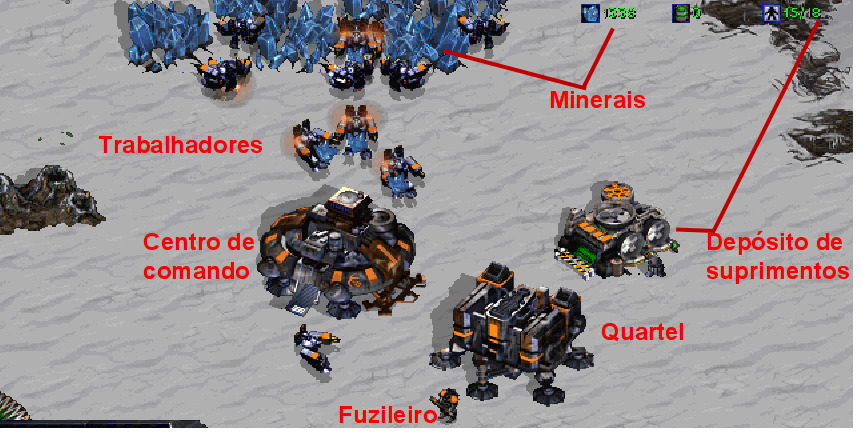
\includegraphics[width=9cm]{img/scsshot.png}}
    \caption{Starcraft screenshot. The command center receives gathered resources and produces workers, the barracks produces marines and supply depots are needed to expand the number of units that can be created.}
    \label{fig:scsshot}
\end{figure}

\section{Experiments}
\label{sec:experiments}




\section{Conclusion}
\label{sec:conclusion}


% An example of a double column floating figure using two subfigures.
% (The subfig.sty package must be loaded for this to work.)
% The subfigure \label commands are set within each subfloat command, the
% \label for the overall figure must come after \caption.
% \hfil must be used as a separator to get equal spacing.
% The subfigure.sty package works much the same way, except \subfigure is
% used instead of \subfloat.
%
%\begin{figure*}[!t]
%\centerline{\subfloat[Case I]\includegraphics[width=2.5in]{subfigcase1}%
%\label{fig_first_case}}
%\hfil
%\subfloat[Case II]{\includegraphics[width=2.5in]{subfigcase2}%
%\label{fig_second_case}}}
%\caption{Simulation results}
%\label{fig_sim}
%\end{figure*}
%
% Note that often IEEE papers with subfigures do not employ subfigure
% captions (using the optional argument to \subfloat), but instead will
% reference/describe all of them (a), (b), etc., within the main caption.


% An example of a floating table. Note that, for IEEE style tables, the 
% \caption command should come BEFORE the table. Table text will default to
% \footnotesize as IEEE normally uses this smaller font for tables.
% The \label must come after \caption as always.
%
%\begin{table}[!t]
%% increase table row spacing, adjust to taste
%\renewcommand{\arraystretch}{1.3}
% if using array.sty, it might be a good idea to tweak the value of
% \extrarowheight as needed to properly center the text within the cells
%\caption{An Example of a Table}
%\label{table_example}
%\centering
%% Some packages, such as MDW tools, offer better commands for making tables
%% than the plain LaTeX2e tabular which is used here.
%\begin{tabular}{|c||c|}
%\hline
%One & Two\\
%\hline
%Three & Four\\
%\hline
%\end{tabular}
%\end{table}


%  Note that, LaTeX2e, unlike IEEE journals/conferences, places
% footnotes above bottom floats. This can be corrected via the \fnbelowfloat
% command of the stfloats package.


% use section* for acknowledgement
\section*{Acknowledgment}


The authors would like to thank...





% trigger a \newpage just before the given reference
% number - used to balance the columns on the last page
% adjust value as needed - may need to be readjusted if
% the document is modified later
%\IEEEtriggeratref{8}
% The "triggered" command can be changed if desired:
%\IEEEtriggercmd{\enlargethispage{-5in}}

% references section

% can use a bibliography generated by BibTeX as a .bbl file
% BibTeX documentation can be easily obtained at:
% http://www.ctan.org/tex-archive/biblio/bibtex/contrib/doc/
% The IEEEtran BibTeX style support page is at:
% http://www.michaelshell.org/tex/ieeetran/bibtex/
%\bibliographystyle{IEEEtran}
% argument is your BibTeX string definitions and bibliography database(s)
%\bibliography{IEEEabrv,../bib/paper}
%
% <OR> manually copy in the resultant .bbl file
% set second argument of \begin to the number of references
% (used to reserve space for the reference number labels box)
\bibliographystyle{IEEEtran}
\bibliography{references}

%\begin{thebibliography}{1}
%
%\bibitem{IEEEhowto:kopka}
%H.~Kopka and P.~W. Daly, \emph{A Guide to \LaTeX}, 3rd~ed.\hskip 1em plus
%  0.5em minus 0.4em\relax Harlow, England: Addison-Wesley, 1999.
%
%\end{thebibliography}




% that's all folks
\end{document}


